
\begin{frame}{The Decremental Consistency Checking Problem: Motivation}
    \begin{figure}
        \centering
        \begin{subfigure}{1.0\textwidth}%
            \centering
            \begin{tikzpicture}
                \tikzstyle{vertex} = [
	shape=circle,  
	draw=blue!50, %draw the border to the node
	fill=blue!20, %fill the space of the node
	thick,
	minimum size=4mm, %minimum size of the nodes
	distance=1cm
];
\pgfarrowsdeclare{directEdge}{directEdge}{%
	\arrowsize=0.2pt
	\advance\arrowsize by .5\pgflinewidth
	\pgfarrowsleftextend{-4\arrowsize-.5\pgflinewidth}
	\pgfarrowsrightextend{.5\pgflinewidth}
}{%
	\arrowsize=1pt
	\advance\arrowsize by .5\pgflinewidth
	\pgfsetdash{}{0pt} % do not dash
	\pgfsetroundjoin % fix join
	\pgfsetroundcap % fix cap
	\pgfpathmoveto{\pgfpointorigin}
	\pgfpathlineto{\pgfpoint{-6\arrowsize}{2.2\arrowsize}}
	\pgfpathlineto{\pgfpoint{-6\arrowsize}{-2.2\arrowsize}}
	\pgfpathclose
	\pgfusepathqfill
}

\begin{scope}[scale=1.0,shift={(-3,0)}]
	\node[vertex](Tw) at (60:2.0cm) {Tw};
	\node[vertex](Mu) at (180:2.0cm) {Mu};
	\node[vertex](Ch) at (-60:2.0cm) {Ch};
\end{scope}

\begin{scope}[scale=1.0,shift={(3,0)}]
	\node[vertex](Lu) at (180:2.0cm) {Lu};
	\node[vertex](Ca) at (-60:2.0cm) {Ca};
	\node[vertex](Te) at (+60:2.0cm) {Te};
\end{scope}

\begin{scope}[scale=1.0,shift={(3,-2)}]
	\node[vertex](Ga) at (180:2.0cm) {Ga};
\end{scope}

%mandatory constraints
\draw[-{Latex[length=2mm,width=3mm]}, line width=0.3mm, color=black]
	(Tw) edge[] (Lu)
	(Ch) edge[] (Lu)
	(Mu) edge[] (Lu)
	(Lu) edge[] (Te)
	(Lu) edge[] (Ca)
;

%first tourist
\draw[-{Latex[length=2mm,width=3mm]}, line width=0.3mm, color=red]
	(Tw) edge[] (Ga)
	(Ga) edge[] (Ca)
	(Ca) edge[dashed] (Te)
;
	
%second tourist
\draw[-{Latex[length=2mm,width=3mm]}, line width=0.3mm, color=green]
	(Tw) edge[dashed] (Mu)
	(Mu) edge[] (Ch)
	(Te) edge[] (Ga)
;

%third tourist
\draw[-{Latex[length=2mm,width=3mm]}, line width=0.3mm, color=blue]
	(Ga) edge[dashed] (Ch)
	(Ch) edge[] (Tw)
;

            \end{tikzpicture}
        \end{subfigure}\\%
        \begin{subfigure}{1.00\textwidth}%
            \centering
            \begin{tikzpicture}
                \tikzstyle{vertex} = [
	shape=circle,  
	fill=black, %fill the space of the node
	thick,
	minimum size=2mm, %minimum size of the nodes
	inner sep=0pt,
	distance=2cm
];
\pgfarrowsdeclare{directEdge}{directEdge}{%
	\arrowsize=0.2pt
	\advance\arrowsize by .5\pgflinewidth
	\pgfarrowsleftextend{-4\arrowsize-.5\pgflinewidth}
	\pgfarrowsrightextend{.5\pgflinewidth}
}{%
	\arrowsize=1pt
	\advance\arrowsize by .5\pgflinewidth
	\pgfsetdash{}{0pt} % do not dash
	\pgfsetroundjoin % fix join
	\pgfsetroundcap % fix cap
	\pgfpathmoveto{\pgfpointorigin}
	\pgfpathlineto{\pgfpoint{-6\arrowsize}{2.2\arrowsize}}
	\pgfpathlineto{\pgfpoint{-6\arrowsize}{-2.2\arrowsize}}
	\pgfpathclose
	\pgfusepathqfill
}

\begin{scope}[scale=1.0,shift={(0,0)}]
	\node[draw=none,label distance=2.5cm,label=below right:\Large{time}](ZERO) at (0, 0) {};
	\node[vertex,label distance=1.6cm,label=above:\Large{Mu}](Mu) at (1, 0) {};
	\node[vertex,label distance=1.6cm,label=above:\Large{Ch}](Ch) at (2, 0) {};
	\node[vertex,label distance=1.6cm,label=above:\Large{Tw}](Tw) at (3, 0) {};
	\node[vertex,label distance=1.6cm,label=above:\Large{Lu}](Lu) at (4, 0) {};
	\node[vertex,label distance=1.6cm,label=above:\Large{Te}](Te) at (5, 0) {};
	\node[vertex,label distance=1.6cm,label=above:\Large{Ga}](Ga) at (6, 0) {};
	\node[vertex,label distance=1.6cm,label=above:\Large{Ca}](Ca) at (7, 0) {};
	\node[draw=none](INF) at (8, 0) {};
\end{scope}

\draw [-directEdge] (ZERO) to[] (INF);




            \end{tikzpicture}
        \end{subfigure}%
    \end{figure}
\end{frame}

\begin{frame}{Definition [Bono, Gerevini, 2018]}
    \vspace{-8pt}
    Given:
	\begin{itemize}
		\item \small{an \textbf{inconsistent temporal CSP} \CSP{} over a class of constraints $\mathcal{C}$};
		\item \small{a \textbf{sequence} $\CSP{}_{0}, ..., \CSP{}_k$ of \TCSPNames{} over $\mathcal{C}$ such that $\CSP{}= \CSP{}_{0}$ and $\CSP{}_i$ is obtained from $\CSP{}_{i-1}$ by making one constraint relaxation in $\CSP{}_{i-1}$, for $i = 1, ..., k$};
	\end{itemize}
	\textbf{\color{blue} Decremental Consistency Checking} is the problem of \textit{iteratively deciding the consistency} of every $\CSP{}_i$ starting from $\CSP{}_1$ until $i = k$ or $\CSP{}_i$ becomes consistent.

    \makebox[\linewidth][c]{\begin{minipage}{1.3\textwidth}
        \begin{figure}
            \centering
            \begin{subfigure}[b]{0.23\textwidth}
                \centering
                \begin{tikzpicture}
                    \tikzstyle{vertex} = [
	shape=circle,  
	draw=blue!50, %draw the border to the node
	fill=blue!20, %fill the space of the node
	thick,
	minimum size=1mm, %minimum size of the nodes
	distance=1cm,
	inner sep=1pt
];

\begin{scope}[scale=1.0,shift={(-1,0)}]
	\node[vertex](Tw) at (90:1.0cm) {Tw};
	\node[vertex](Mu) at (180:0.5cm) {Mu};
	\node[vertex](Ch) at (-90:1.0cm) {Ch};
\end{scope}

\begin{scope}[scale=1.0,shift={(0.8,0)}]
	\node[vertex](Lu) at (180:1.0cm) {Lu};
	\node[vertex](Ca) at (-90:1.0cm) {Ca};
	\node[vertex](Te) at (+90:1.0cm) {Te};
\end{scope}

\begin{scope}[scale=1.0,shift={(0.9,-1)}]
	\node[vertex](Ga) at (180:1.0cm) {Ga};
\end{scope}

%mandatory constraints
\draw[-{Latex[length=2mm,width=3mm]}, line width=0.3mm, color=black]
	(Tw) edge[] (Lu)
	(Ch) edge[] (Lu)
	(Mu) edge[] (Lu)
	(Lu) edge[] (Te)
	(Lu) edge[] (Ca)
;

%first tourist
\draw[-{Latex[length=2mm,width=3mm]}, line width=0.3mm, color=red]
	(Tw) edge[] (Ga)
	(Ga) edge[] (Ca)
	(Ca) edge[] (Te)
;
	
%second tourist
\draw[-{Latex[length=2mm,width=3mm]}, line width=0.3mm, color=green]
	(Tw) edge[] (Mu)
	(Mu) edge[] (Ch)
	(Te) edge[] (Ga)
;

%third tourist
\draw[-{Latex[length=2mm,width=3mm]}, line width=0.3mm, color=blue]
	(Ga) edge[] (Ch)
	(Ch) edge[] (Tw)
;

                \end{tikzpicture}
                \caption{$\CSP{}_{0}$}
            \end{subfigure}%
            \begin{subfigure}[b]{0.23\textwidth}
                \centering
                \begin{tikzpicture}
                    \tikzstyle{vertex} = [
	shape=circle,  
	draw=blue!50, %draw the border to the node
	fill=blue!20, %fill the space of the node
	thick,
	minimum size=1mm, %minimum size of the nodes
	distance=1cm,
	inner sep=1pt
];

\begin{scope}[scale=1.0,shift={(-1,0)}]
	\node[vertex](Tw) at (90:1.0cm) {Tw};
	\node[vertex](Mu) at (180:0.5cm) {Mu};
	\node[vertex](Ch) at (-90:1.0cm) {Ch};
\end{scope}

\begin{scope}[scale=1.0,shift={(0.8,0)}]
	\node[vertex](Lu) at (180:1.0cm) {Lu};
	\node[vertex](Ca) at (-90:1.0cm) {Ca};
	\node[vertex](Te) at (+90:1.0cm) {Te};
\end{scope}

\begin{scope}[scale=1.0,shift={(0.9,-1)}]
	\node[vertex](Ga) at (180:1.0cm) {Ga};
\end{scope}

%mandatory constraints
\draw[-{Latex[length=2mm,width=3mm]}, line width=0.3mm, color=black]
	(Tw) edge[] (Lu)
	(Ch) edge[] (Lu)
	(Mu) edge[] (Lu)
	(Lu) edge[] (Te)
	(Lu) edge[] (Ca)
;

%first tourist
\draw[-{Latex[length=2mm,width=3mm]}, line width=0.3mm, color=red]
	(Tw) edge[] (Ga)
	(Ga) edge[] (Ca)
;
	
%second tourist
\draw[-{Latex[length=2mm,width=3mm]}, line width=0.3mm, color=green]
	(Tw) edge[] (Mu)
	(Mu) edge[] (Ch)
	(Te) edge[] (Ga)
;

%third tourist
\draw[-{Latex[length=2mm,width=3mm]}, line width=0.3mm, color=blue]
	(Ga) edge[] (Ch)
	(Ch) edge[] (Tw)
;

                \end{tikzpicture}
                \caption{$\CSP{}_{1}$}
            \end{subfigure}%
            \begin{subfigure}[b]{0.23\textwidth}
                \centering
                \begin{tikzpicture}
                    \tikzstyle{vertex} = [
	shape=circle,  
	draw=blue!50, %draw the border to the node
	fill=blue!20, %fill the space of the node
	thick,
	minimum size=1mm, %minimum size of the nodes
	distance=1cm,
	inner sep=1pt
];

\begin{scope}[scale=1.0,shift={(-1,0)}]
	\node[vertex](Tw) at (90:1.0cm) {Tw};
	\node[vertex](Mu) at (180:0.5cm) {Mu};
	\node[vertex](Ch) at (-90:1.0cm) {Ch};
\end{scope}

\begin{scope}[scale=1.0,shift={(0.8,0)}]
	\node[vertex](Lu) at (180:1.0cm) {Lu};
	\node[vertex](Ca) at (-90:1.0cm) {Ca};
	\node[vertex](Te) at (+90:1.0cm) {Te};
\end{scope}

\begin{scope}[scale=1.0,shift={(0.9,-1)}]
	\node[vertex](Ga) at (180:1.0cm) {Ga};
\end{scope}

%mandatory constraints
\draw[-{Latex[length=2mm,width=3mm]}, line width=0.3mm, color=black]
	(Tw) edge[] (Lu)
	(Ch) edge[] (Lu)
	(Mu) edge[] (Lu)
	(Lu) edge[] (Te)
	(Lu) edge[] (Ca)
;

%first tourist
\draw[-{Latex[length=2mm,width=3mm]}, line width=0.3mm, color=red]
	(Tw) edge[] (Ga)
	(Ga) edge[] (Ca)
;
	
%second tourist
\draw[-{Latex[length=2mm,width=3mm]}, line width=0.3mm, color=green]
	(Mu) edge[] (Ch)
	(Te) edge[] (Ga)
;

%third tourist
\draw[-{Latex[length=2mm,width=3mm]}, line width=0.3mm, color=blue]
	(Ga) edge[] (Ch)
	(Ch) edge[] (Tw)
;

                \end{tikzpicture}
                \caption{$\CSP{}_{2}$}
            \end{subfigure}%
            \begin{subfigure}[b]{0.23\textwidth}
                \centering
                \begin{tikzpicture}
                    \tikzstyle{vertex} = [
	shape=circle,  
	draw=blue!50, %draw the border to the node
	fill=blue!20, %fill the space of the node
	thick,
	minimum size=1mm, %minimum size of the nodes
	distance=1cm,
	inner sep=1pt
];

\begin{scope}[scale=1.0,shift={(-1,0)}]
	\node[vertex](Tw) at (90:1.0cm) {Tw};
	\node[vertex](Mu) at (180:0.5cm) {Mu};
	\node[vertex](Ch) at (-90:1.0cm) {Ch};
\end{scope}

\begin{scope}[scale=1.0,shift={(0.8,0)}]
	\node[vertex](Lu) at (180:1.0cm) {Lu};
	\node[vertex](Ca) at (-90:1.0cm) {Ca};
	\node[vertex](Te) at (+90:1.0cm) {Te};
\end{scope}

\begin{scope}[scale=1.0,shift={(0.9,-1)}]
	\node[vertex](Ga) at (180:1.0cm) {Ga};
\end{scope}

%mandatory constraints
\draw[-{Latex[length=2mm,width=3mm]}, line width=0.3mm, color=black]
	(Tw) edge[] (Lu)
	(Ch) edge[] (Lu)
	(Mu) edge[] (Lu)
	(Lu) edge[] (Te)
	(Lu) edge[] (Ca)
;

%first tourist
\draw[-{Latex[length=2mm,width=3mm]}, line width=0.3mm, color=red]
	(Tw) edge[] (Ga)
	(Ga) edge[] (Ca)
;
	
%second tourist
\draw[-{Latex[length=2mm,width=3mm]}, line width=0.3mm, color=green]
	(Mu) edge[] (Ch)
	(Te) edge[] (Ga)
;

%third tourist
\draw[-{Latex[length=2mm,width=3mm]}, line width=0.3mm, color=blue]
	(Ch) edge[] (Tw)
;

                \end{tikzpicture}
                \caption{$\CSP{}_{3}$}
            \end{subfigure}
        \end{figure}
    \end{minipage}}

    If the \TCSPNames{} are all over \PAName{} (\OrdHornName{}), the problem is called \DPSATProblemName{} (\DOHSATProblemName{}).
\end{frame}

\begin{frame}{\PSATProblemName{} [van Beek, 1992]}
    How to solve the problem of \textit{statically} checking the consistency of a \TCSPName{} \CSP{} over \PAName{} (\PSATProblemName{})?

    \begin{itemize}
        \item Compute the \textit{Strongly Connected Components} (\SCCNames{}) of the \tlGraphName{} of \CSP{};
        \item Edge labeled either with \squote{$<$} or \squote{$\noteq{}$} is in a \SCCName{} subgraph $\Leftrightarrow$ \CSP{} inconsistent;
    \end{itemize}

    \begin{figure}
        \begin{tikzpicture}
            \tikzstyle{vertex}=[shape=circle, fill=blue!20, draw=blue!50, thick, minimum size=2mm, inner sep=5pt, distance=1.7cm];

            \begin{scope}[scale=1.0, shift={(0,0)}]
                \node at (0,2.1cm) {$\SCC{}_{1}$};
                \draw[fill=red!20, draw=red!50] (0,0) circle (1.8cm);
                \node[vertex](A) at (35:1.3cm) {$a$};
                \node[vertex](B) at (155:1.3cm) {$b$};
                \node[vertex](C) at (275:1.3cm) {$c$};
            \end{scope}

            \begin{scope}[scale=1.0, shift={(7,0)}]
                \node at (0,2.1cm) {$\SCC{}_{3}$};
                \draw[fill=red!20, draw=red!50] (0,0) circle (1.9cm);
                \node[vertex](D) at (17:1.4cm) {$d$};
                \node[vertex](E) at (107:1.4cm) {$e$};
                \node[vertex](F) at (197:1.4cm) {$f$};
                \node[vertex](G) at (287:1.4cm) {$g$};
            \end{scope}

            \begin{scope}[scale=1.0, shift={(3.5,0)}]
                \node at (0,2.1cm) {$\SCC{}_{2}$};
                \draw[fill=green!20, draw=green!50, rotate=10] (0,0) circle (1.1cm and 1.8cm);
                \node[vertex](H) at (100:1.3cm) {$h$};
                \node[vertex](I) at (280:1.3cm) {$i$};
            \end{scope}

            \draw[-{Latex[length=2mm,width=3mm]}, line width=0.3mm]
                (A) edge[color=red, line width=0.5mm] node[below] {$<$} (B)
                (B) edge node[above] {$\leq$} (C)
                (C) edge node[left] {$\leq$} (A)
            ;

            \draw[-{Latex[length=2mm,width=3mm]}, line width=0.3mm]
                (D) edge[color=red, line width=0.5mm] node[below] {$<$} (E)
                (E) edge[color=red, line width=0.5mm] node[right] {$<$} (F)
                (F) edge[color=red, line width=0.5mm] node[above] {$<$} (G)
                (G) edge[bend left] node[left] {$\leq$} (D)
                (D) edge[bend left] node[left] {$\leq$} (G)
            ;

            \draw[-.]
                (F) edge[color=red, line width=0.5mm] node[above] {$\not =$} (D)
            ;

            \draw[-{Latex[length=2mm,width=3mm]}, line width=0.3mm]
                (H) edge[bend left] node[left] {$\leq$} (I)
                (I) edge[bend left] node[left] {$\leq$} (H)
            ;

            \draw[-{Latex[length=2mm,width=3mm]}, line width=0.3mm]
                (A) edge node[above, yshift=1pt] {$<$} (H)
                (I) edge node[above, yshift=1pt] {$\leq$} (F)
            ;
        \end{tikzpicture}
    \end{figure}
\end{frame}

\begin{frame}{Solving \DPSATProblemName{}}
    Proposed algorithm \DPASATAlgorithmName{}:
    \begin{itemize}
        \item Decremental variant of \PSATProblemName{};
        \item Compute useful metadata at the first constraint relaxation allowing us to quickly compute consistency (\ie{} problematic \SCCNames{} and edges in \SCCNames{} with label $\in \{ \squote{<}, \squote{\noteq{}} \}$);
        \item Mantain such metadata over the sequence of \TCSPNames{};
    \end{itemize}
\end{frame}

\begin{frame}{Solving \DOHSATProblemName{}}
    \IAName{} algebra is intractable $\Rightarrow$ consider a subalgebra which is tractable (\OrdHornName{})

    \DOHSATProblemName{}:
    \begin{itemize}
        \item Each \TCSPName{} \IACSP{} can be seen as $\piOne{\IACSP{}} \cup \piTwo{\IACSP{}}$ ($\piOne{\IACSP{}}$ = \TCSPName{} over \PAName{}; $\piTwo{\IACSP{}}$: set of at most binary disjunctions where each disjunct is of the form $p \{=, \leq, \noteq{} \} q$ and at least one of them is $p \noteq{} q$)
    \end{itemize}

    Proposed algorithm \DOHSATAlgorithmName{}:
    \begin{itemize}
        \item Decremental variant of \OHSATAlgorithmName{} ([Gerevini, 2005]);
        \item Use \DPASATAlgorithmName{} to manage $\piOne{\IACSP{}}$;
        \item Compute useful metadata as soon $\piOne{\IACSP{}}$ becomes consistent allowing us to reuse previous \OHSATAlgorithmName{} inferences;
        \item Mantain such metadata over the sequence of \TCSPNames{};
    \end{itemize}
\end{frame}

\begin{frame}{Experimental results}
    \begin{itemize}
        \item Each point represents the average CPU-time over 30 instances used by algorithms to solve the decremental problem;
        \item VB (\OHSATAlgorithmName{} and PC) is the \stateofart{} algorithm statically checking consistency of \TCSPName{} over \PAName{} (\OrdHornName{});
        \item \textit{Sparse} graphs are graphs with $\lfloor n \log_2{n} \rfloor$ constraints;
    \end{itemize}

    \begin{figure}
        \centering
        \begin{subfigure}{0.49\textwidth}
            \centering
            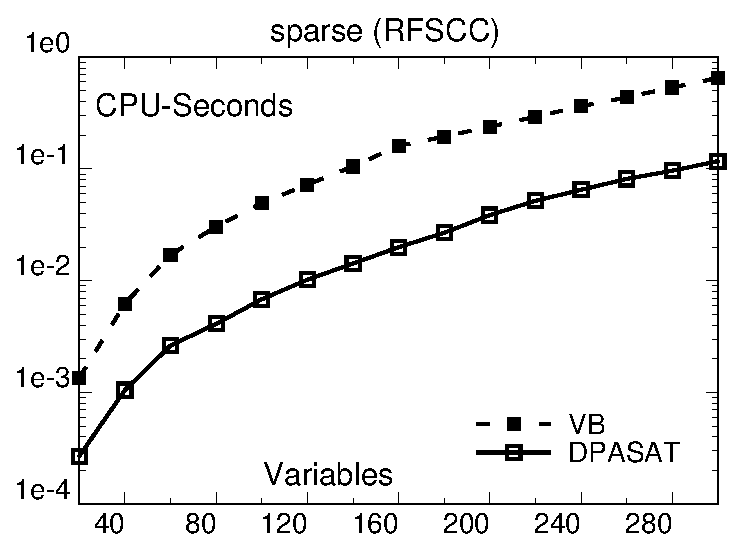
\includegraphics[width=1.0\textwidth]{src/images/temporal-reasoning/dpasat}
        \end{subfigure}%
        \begin{subfigure}{0.49\textwidth}
            \centering
            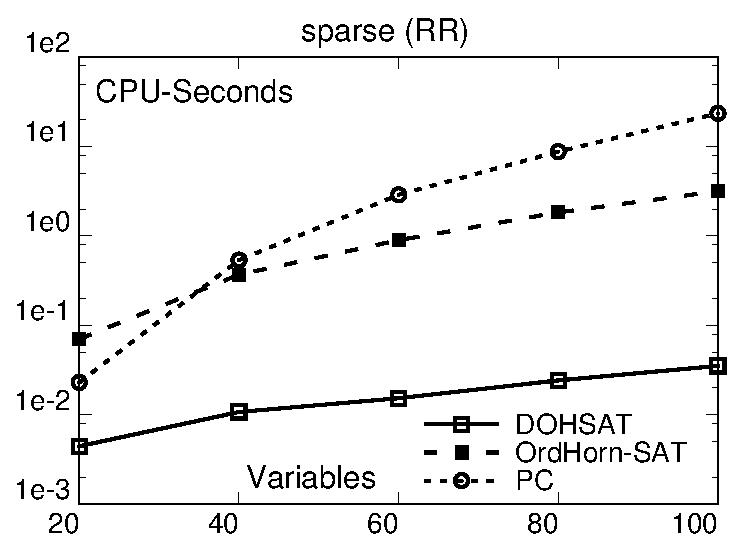
\includegraphics[width=1.0\textwidth]{src/images/temporal-reasoning/dohsat}
        \end{subfigure}
    \end{figure}
\end{frame}